\documentclass[man,floatsintext]{apa6}
\usepackage{lmodern}
\usepackage{amssymb,amsmath}
\usepackage{ifxetex,ifluatex}
\usepackage{fixltx2e} % provides \textsubscript
\ifnum 0\ifxetex 1\fi\ifluatex 1\fi=0 % if pdftex
  \usepackage[T1]{fontenc}
  \usepackage[utf8]{inputenc}
\else % if luatex or xelatex
  \ifxetex
    \usepackage{mathspec}
  \else
    \usepackage{fontspec}
  \fi
  \defaultfontfeatures{Ligatures=TeX,Scale=MatchLowercase}
\fi
% use upquote if available, for straight quotes in verbatim environments
\IfFileExists{upquote.sty}{\usepackage{upquote}}{}
% use microtype if available
\IfFileExists{microtype.sty}{%
\usepackage{microtype}
\UseMicrotypeSet[protrusion]{basicmath} % disable protrusion for tt fonts
}{}
\usepackage{hyperref}
\hypersetup{unicode=true,
            pdftitle={Reproduing analysis of: Unlearning implicit social biases during sleep (2015)},
            pdfauthor={Richard Troise},
            pdfkeywords={social biases, slow-wave sleep},
            pdfborder={0 0 0},
            breaklinks=true}
\urlstyle{same}  % don't use monospace font for urls
\usepackage{graphicx,grffile}
\makeatletter
\def\maxwidth{\ifdim\Gin@nat@width>\linewidth\linewidth\else\Gin@nat@width\fi}
\def\maxheight{\ifdim\Gin@nat@height>\textheight\textheight\else\Gin@nat@height\fi}
\makeatother
% Scale images if necessary, so that they will not overflow the page
% margins by default, and it is still possible to overwrite the defaults
% using explicit options in \includegraphics[width, height, ...]{}
\setkeys{Gin}{width=\maxwidth,height=\maxheight,keepaspectratio}
\IfFileExists{parskip.sty}{%
\usepackage{parskip}
}{% else
\setlength{\parindent}{0pt}
\setlength{\parskip}{6pt plus 2pt minus 1pt}
}
\setlength{\emergencystretch}{3em}  % prevent overfull lines
\providecommand{\tightlist}{%
  \setlength{\itemsep}{0pt}\setlength{\parskip}{0pt}}
\setcounter{secnumdepth}{0}
% Redefines (sub)paragraphs to behave more like sections
\ifx\paragraph\undefined\else
\let\oldparagraph\paragraph
\renewcommand{\paragraph}[1]{\oldparagraph{#1}\mbox{}}
\fi
\ifx\subparagraph\undefined\else
\let\oldsubparagraph\subparagraph
\renewcommand{\subparagraph}[1]{\oldsubparagraph{#1}\mbox{}}
\fi

%%% Use protect on footnotes to avoid problems with footnotes in titles
\let\rmarkdownfootnote\footnote%
\def\footnote{\protect\rmarkdownfootnote}


  \title{Reproduing analysis of: Unlearning implicit social biases during sleep
(2015)}
    \author{Richard Troise\textsuperscript{1}}
    \date{}
  
\shorttitle{Unlearning implicit social biases during sleep}
\affiliation{
\vspace{0.5cm}
\textsuperscript{1} Brooklyn College}
\keywords{social biases, slow-wave sleep\newline\indent Word count: X}
\usepackage{csquotes}
\usepackage{upgreek}
\captionsetup{font=singlespacing,justification=justified}

\usepackage{longtable}
\usepackage{lscape}
\usepackage{multirow}
\usepackage{tabularx}
\usepackage[flushleft]{threeparttable}
\usepackage{threeparttablex}

\newenvironment{lltable}{\begin{landscape}\begin{center}\begin{ThreePartTable}}{\end{ThreePartTable}\end{center}\end{landscape}}

\makeatletter
\newcommand\LastLTentrywidth{1em}
\newlength\longtablewidth
\setlength{\longtablewidth}{1in}
\newcommand{\getlongtablewidth}{\begingroup \ifcsname LT@\roman{LT@tables}\endcsname \global\longtablewidth=0pt \renewcommand{\LT@entry}[2]{\global\advance\longtablewidth by ##2\relax\gdef\LastLTentrywidth{##2}}\@nameuse{LT@\roman{LT@tables}} \fi \endgroup}



\authornote{Add complete departmental affiliations for each
author here. Each new line herein must be indented, like this line.

Enter author note here.

Correspondence concerning this article should be addressed to Richard
Troise, Postal address. E-mail:
\href{mailto:my@email.com}{\nolinkurl{my@email.com}}}

\abstract{
There is evidence by Hu et al. (2015) on the unlearning of social bias
by reinforcing a counterbias behavior during slow-wave/REM sleep - the
optimal time frame to consolidate new memories. The reproduced analysis
pertains to the interaction of cued and uncued reduction bias before
sleep (prenap), then, one week later (delayed). A power analysis shows
that the original effect size may only be observed approximately half
the time on average.


}

\begin{document}
\maketitle

The experiment on unlearning social bias shows the relevance of sleep
playing a role in the dissaption of the pre-existing implicit bias, Hu
et al. (2015). The rationale comes from auditory information reinforcing
learning behavior during slow wave sleep, causing a targeted memory
reactivation. As a result of the auditory cue, counterbias behavior in
participants was expected to increase. In addition, the memory
reactivation should result in a sustained reduction in social bias, in
that the measured bias does not differ between prenap and delay. The
implications of such an effect may be relevant for unlearning other
unwanted habits. The original data was downloaded from
\href{https://osf.io/b7x8q/}{https://osf.io/b3k9a/}

second citation Muller and Barton (1989)

\section{Methods}\label{methods}

\subsection{Participants}\label{participants}

As stated in experiment, there were 40 participants recruited but only
38 were present for all groups.

\subsection{Material}\label{material}

The details of the experiment can be found in Hu et al. (2015).

\subsection{Procedure}\label{procedure}

The 38 participants experienced four conditions:

\subsection{Data analysis}\label{data-analysis}

We used R (Version 3.5.0; R Core Team, 2018) and the R-packages
\emph{dplyr} (Version 0.8.0.1; Wickham, François, Henry, \& Müller,
2019), \emph{papaja} (Version 0.1.0.9842; Aust \& Barth, 2018), and
\emph{xtable} (Version 1.8.3; Dahl, Scott, Roosen, Magnusson, \&
Swinton, 2018) for all our analyses.

\section{Results}\label{results}

Figure 2: Results of 2x2 repeated measured ANOVA

\begin{tabular}{l|r|r|r|r|r}
\hline
  & Df & Sum Sq & Mean Sq & F value & Pr(>F)\\
\hline
Residuals & 37 & 9.4853844 & 0.2563617 & NA & NA\\
\hline
cue\_factor & 1 & 0.0929324 & 0.0929324 & 0.3355098 & 0.5659427\\
\hline
Residuals & 37 & 10.2485769 & 0.2769886 & NA & NA\\
\hline
time\_factor & 1 & 0.8440958 & 0.8440958 & 5.7634410 & 0.0215060\\
\hline
Residuals & 37 & 5.4189059 & 0.1464569 & NA & NA\\
\hline
cue\_factor:time\_factor & 1 & 0.3290260 & 0.3290260 & 4.6718467 & 0.0372022\\
\hline
Residuals & 37 & 2.6058138 & 0.0704274 & NA & NA\\
\hline
\end{tabular}

From figure 1. 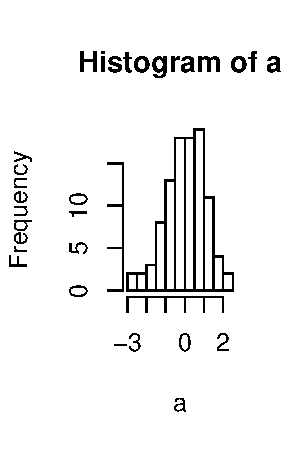
\includegraphics{first_apa_files/figure-latex/fig1-1.pdf}

\section{Discussion}\label{discussion}

\newpage

\section{References}\label{references}

\begingroup
\setlength{\parindent}{-0.5in} \setlength{\leftskip}{0.5in}

\hypertarget{refs}{}
\hypertarget{ref-R-papaja}{}
Aust, F., \& Barth, M. (2018). \emph{papaja: Create APA manuscripts with
R Markdown}. Retrieved from \url{https://github.com/crsh/papaja}

\hypertarget{ref-R-xtable}{}
Dahl, D. B., Scott, D., Roosen, C., Magnusson, A., \& Swinton, J.
(2018). \emph{Xtable: Export tables to latex or html}. Retrieved from
\url{https://CRAN.R-project.org/package=xtable}

\hypertarget{ref-Hu1013}{}
Hu, X., Antony, J. W., Creery, J. D., Vargas, I. M., Bodenhausen, G. V.,
\& Paller, K. A. (2015). Unlearning implicit social biases during sleep,
\emph{348}(6238), 1013--1015.
doi:\href{https://doi.org/10.1126/science.aaa3841}{10.1126/science.aaa3841}

\hypertarget{ref-Keith1989}{}
Muller, K. E., \& Barton, C. N. (1989). Approximate power for
repeated-measures anova lacking sphericity. \emph{Journal of the
American Statistical Association}, \emph{84}(406), 549--555.
doi:\href{https://doi.org/10.1080/01621459.1989.10478802}{10.1080/01621459.1989.10478802}

\hypertarget{ref-R-base}{}
R Core Team. (2018). \emph{R: A language and environment for statistical
computing}. Vienna, Austria: R Foundation for Statistical Computing.
Retrieved from \url{https://www.R-project.org/}

\hypertarget{ref-R-dplyr}{}
Wickham, H., François, R., Henry, L., \& Müller, K. (2019). \emph{Dplyr:
A grammar of data manipulation}. Retrieved from
\url{https://CRAN.R-project.org/package=dplyr}

\endgroup


\end{document}
